
\subsection{Differential expression and accessibility analyses}

Read counts for each sample were converted to counts per million (CPM) and normalized using TMM normalization (\textit{edgeR}). Windows with > 70 \% of samples with CPM $\leq$ 1 were removed. Differentially expressed genes and accessible chromatin windows were determined using \textit{limma} \citep{limma} with the linear model:
\begin{equation}
y_{i} = \mu + \text{strain}_{i} + \text{batch}_{i} + \text{tissue}_{i} + \varepsilon_{i},
\label{eq:limma_model}
\end{equation}
where $y_{i}$ is the TMM-normalized CPM value in $\text{tissue}_{i}$ (lung, liver, or kidney tissue) from individual $i$. $\mu$ is the intercept, representing the overall mean; $\text{batch}_{i}$ is effect of sequencing center; $\text{strain}_i$ is the strain-specific effect; and $\varepsilon_{i}$ is an error term, with $\varepsilon_{i} \sim \text{N}(0, \sigma^{2})$.

To account for mean-variance relationships in gene expression and chromatin accessibility data, precision weights were calculated using the \textit{limma} function \textit{voom} and incorporated into the linear modeling procedure. The p-values were adjusted using an FDR procedure \citep{Benjamini1995}, and differentially expressed genes and accessible chromatin windows were called based on the q-value $\le$ 0.01 and log$_{2}$ fold-change $\geq$ 1. Adjacent significantly differential chromatin windows in the same direction were merged with a p-value computed using Simes' method \citep{Sarkar1997}, and chromatin regions were re-evaluated for significance using the Simes p-values.

\subsection{Gene set association analysis}

GSAASeqSP \citep{Xiong2014} with Reactome Pathway Database annotations (July 24, 2015 release) was used to identify biological pathways enriched with differentially expressed genes or accessible chromatin. For genes, gene lists were provided as input to GSAASeqSP along with a weight for each gene $g$, calculated as:
\begin{equation}
\text{weight}_{g} = \text{sign}(\text{fc}_{g}) * (1-q_{g}),
\label{eq:gene_weighting}
\end{equation}
where $\text{sign}(\text{fc}_{g})$ is the sign of the expression fold change, and $q_{g}$ is the FDR-adjusted p-value. Pathways with gene sets of cardinality < 15 or > 500 were excluded. For chromatin accessibility, each region was mapped to a gene using GREAT v3.0.0 (\textit{basal plus extension} mode, \textit{5 kb upstream}, \textit{1 kb downstream}, and no distal extension). Each gene was associated with the chromatin region with the most significant FDR-adjusted q-value and gene weights were calculated as above with $\text{sign}(\text{fc}_{g})$, the sign of chromatin accessibility fold-change and $q_{g}$ the FDR-adjusted q-value of the chromatin region representing gene $g$.

\subsection{QTL analysis}

A single locus approach to QTL mapping was used for both gene expression and chromatin accessibility. The CC mice have well-characterized founder haplotypes, allowing the association analysis to be haplotype-based, also referred to as interval mapping or linkage analysis \citep{Lander1989}. Assessing association between haplotype descent and phenotype has advantages to variant association, such as implicitly modeling multiple local variants simultaneously and more closely reflecting the linkage disequilibrium (LD) decay. Because haplotype state is not directly observed but rather probabilistically inferred \citep{Lander1987,Mott2000,Liu2010,Fu2012,Gatti2014,Zheng2015}, formal interval mapping requires an computationally inefficient Expectation-Maximization (EM) algorithm \citep{Dempster1977}. A computationally efficient regression approximation \citep{Haley1992,Martinez1992} is commonly used instead for multiparental populations (MPP) \citep{Valdar2006a,Valdar2009,Svenson2012,Baud2013,Baud2014}, including the CC \citep{Aylor2011,Kelada2016,Mosedale2017,Donoghue2017}. This efficiency is particularly important in the context of a study of genome-wide molecular phenotypes.

\begin{table*}[h]
\renewcommand{\familydefault}{\sfdefault}\normalfont
\begin{tableminipage}{\textwidth}
\captionsetup{width=\textwidth}
\centering
\caption{\bf QTL mapping procedures
\label{tab:qtl_procedures}}
\end{tableminipage}
\begin{tableminipage}{\textwidth}
\begin{tabularx}{\textwidth}{l | cccc}
\hline 
Procedure & QTL type & FWER control & FDR control & QTL per trait \\
\hline
Method 1 & local \& distal & genome-wide & yes & $\ge$ 1 \\
Method 2 & local \& intra-chromosomal distal & chromosome-wide & yes & 1 \\
Method 3 & local & genome \& chromosome-wide & no & 1 \\
\hline
\end{tabularx}
\end{tableminipage}
\end{table*}

\subsubsection{General QTL model.}
For a genome scan, the alternative model is fit at positions across the genome and compared to the null model of no locus effect. The general alternative model for gene expression and chromatin accessibility is the same: 
\begin{equation}
y_{i} = \mu + \text{QTL}_{i} + \text{batch}_{i} + \varepsilon_{i},
\label{eq:alternative_model}
\end{equation}
where $y_{i}$ is the trait, either levels of gene expression or chromatin accessibility for individual $i$. $\mu$ is an intercept term, representing the sample mean. $\text{QTL}_{i}$ is the genetic locus effect, here fit according to an additive fixed effects model. The effect of sequencing center is modeled as the covariate $\text{batch}_{i}$. $\varepsilon_{i}$ is the error term for individual $i$, such that $\varepsilon_{i} \sim \text{N}(0, \sigma^{2})$. $y$ are transformed to better satisfy the regression assumption that the residuals are normally distributed; here we take the normal quantiles from the ranks of the trait, in order to be strongly reduce the influence of potential extreme observations in a sample of 47 individuals. The null model is the same for all tested loci and is equivalent to Eq \ref{eq:alternative_model} with $\text{QTL}_{i} = 0$ for all individuals. The two models are compared statistically at each position, and summarized with an F-test p-value. QTL are detected if the improvement in fit of the alternative model compared to the null model surpasses a set threshold of significance.

\subsubsection{Significance thresholds.}
Thresholds of significance in the context of genome-wide scans for a large number of traits need to account for the heavy multiple testing burden. In order to efficiently detect QTL, we use three procedures to define statistical significance over varying stringency, allowing greater leniency for putative proximal genetic regulators. These procedures address the family-wide error rate (FWER) and false discovery rate (FDR) differently.

At the level of a single trait, FWER is the probability of a false positive across all tests that are performed. The FWER is controlled through adjustment of an observed -$\log_{10}$ p-value (logP) through 1,000 permutations of the trait, producing an FWER-adjusted p-value (permP). This adjustment can be performed for genome-wide and more lenient chromosome-wide significance.

To account for multiple testing over many traits, an FDR adjustment \citep{Benjamini1995} can be used to produce q-values, which are interpreted as the probability that a detected QTL is a false discovery. See \textbf{Appendix A} for greater detail on the control of FWER and FDR. 

\subsubsection{Mapping procedures.} Three mapping procedures were used to detect QTL, each with unique features. They are as follows:
\begin{enumerate}[label = \method{{\arabic*:}}]
\setlength{\itemindent}{3em}
	\item Multi-stage conditional regression with genome-wide FWER and FDR control. This procedure is the most statistically stringent, can identify both local and distal-QTL, and potentially multiple QTL per trait in an unbiased FDR control.
    \item Single-stage regression with chromosome-wide FWER and FDR control. This procedure is oriented towards identification of local-QTL by using the much more lenient chromosome-wide FWER adjustment. Putative distal-QTL that are located on the same chromosome as the target but are not proximal to the trait's genomic coordinate are also leniently detected, referred to here as intra-chromosomal distal-QTL.
    \item Single-stage regression with genome-wide and chromosome-wide FWER control. This procedure only detects local-QTL, leveraging strong biological precedent for local genetic regulation to reduce the significance threshold. FWER adjustment, either at genome or chromosome-wide levels, is performed for the maximum logP in the local window (defined here as 10 Mb upstream or downstream of target's coordinate), without FDR control.
\end{enumerate}

See \textbf{Table \ref{tab:qtl_procedures}} for simple breakdowns of the three procedures and \textbf{Appendix B} for greater detail on each.

\subsubsection{QTL founder allele effects and effect size.} 

The founder allele effects at a QTL, as fit in the mapping model (Eq \ref{eq:alternative_model}), can help distinguish which genetic variants drive an observed QTL. However, these effects, when pulled directly from the mapping procedures, are comprised of a vector with one fixed effect regression coefficient per founder strain, and can be unstable when there are few observations per founder strain contribution at a locus, resulting in artificially extreme effects \citep{Zhang2014}. To conservatively constrain the effect estimates, the model in Eq \ref{eq:alternative_model} was re-fit at the detected QTL, but with the QTL effect as a random effect vector with corresponding variance component \citep{Wei2016}, such that $\text{QTL}_{i} = \bx_{i}\bbeta$ with $\bbeta \sim \text{N}(\bzero, \bI\tausq)$. $\bx_{i}$ is the founder haplotype dosage vector for individual $i$ at the QTL, $\bbeta$ is the QTL effect vector, and $\tausq$ is the variance component corresponding to the QTL effect vector. The best linear unbiased predictors of the allele effects [$\widehat{\bbeta}_{\text{BLUP}}$] \citep{Robinson1991} were calculated and used for further comparison of QTL across tissues. A point estimate of the proportion of the variance explained by the QTL effect is calculated as:
\begin{equation}
    \text{QTL effect size} = \frac{\widehat{\tau^{2}}}{\widehat{\tau^{2}} + \widehat{\sigma^{2}}},
    \label{eq:effect_size}
\end{equation} which is referred to as the QTL effect size and also used to compare and summarize QTL findings. 

\subsubsection{Cross-tissue comparison of QTL.}

To evaluate patterns of the genetic regulation of gene expression and chromatin accessibility across tissues, correlations between the founder allele effects of QTL that map to approximately the same region of the genome for the same traits but in different tissues were calculated. Pairs of local-QTL were required to both be detected within the 20 Mb window around the gene TSS or the chromatin window midpoint. For distal-QTL, the QTL positions had to be within 10 Mb of each other. All detected QTL were considered, including QTL from Methods 1 and 2 controlled at an FDR of 0.2, allowing for consistent signal across tissues to provide further evidence for putative QTL with marginal significance within a single tissue.

For a pair of matched QTL $j$ and $k$ from different tissues, the Pearson correlation coefficient was calculated as $r_{jk} = \text{cor}(\widehat{\bbeta}_{\text{BLUP}}^{j}, \widehat{\bbeta}_{\text{BLUP}}^{k})$. $\widehat{\bbeta}_{\text{BLUP}}$ represent 8-element vectors, thus corresponding $r$ are distributed such that $\frac{r\sqrt{6}}{1 - r^{2}} \sim t_{6}$ according to the null model of independent variables. Testing the alternative models that $r_{jk} > 0$ and $r_{jk} < 0$ were performed for each pair of QTL, producing p-values. An FDR procedure (Benjamini-Hochburg) was then used to retrieve two q-values per QTL pair, $q_{ij}^{\{r > 0\}}$ and $q_{ij}^{\{r < 0\}}$, which were used to classify pairs of QTL as being significantly correlated or anti-correlated, respectively. 

\subsubsection{Variant association.}

Variant association was performed within the genomic regions surrounding overlapping QTL in order to detect similarities and differences patterns of association between tissues. Variant genotypes from Build38 were obtained using the ISVdb \citep{Oreper2017} for the CC strains, which were converted to Build37 coordinates with the liftOver tool \citep{Lawrence2009}. Variants were filtered out if they had minor allele frequencies below 0.1 or were not genotyped in one of the CC founder strains to avoid artificially high signals.

\subsection{Mediation analysis}

Detection of mediator relationship is dependent on a number of assumptions about the underlying variables, their relationships, and the directionality of those relationships, many of which cannot be satisfied in systems far less complex than that between chromatin state and gene transcription in living organisms. However, evidence that is consistent with chromatin state acting as a mediator of gene expression is supportive of the hypothesis that chromatin state plays a key role in the regulation of gene transcription.

\cite{Baron1986} give a description of the relationships that need be tested to declare mediation. For this study, simple models that consist of three variables are used: the independent variable X, the mediator M, and the dependent variable Y \citep{MacKinnon2007}. Superscripts are used to indicate whether a variable is the QTL, chromatin accessibility at site $k$ ($\text{C}_{k}$), or expression of gene $j$ ($\text{G}_{j}$) in the model. When an eQTL is detected, the following relationship is supported:
\begin{equation}
\text{X}\textsuperscript{QTL} \quad \rightarrow \quad \text{Y}^{\text{G}_{j}}
\label{rel:eQTL}
\end{equation}
When cQTL or proximal eQTL to distal-eQTL are detected, a similar relationship is detected:
\begin{equation}
\text{X}\textsuperscript{QTL} \quad \rightarrow \quad \text{M}
\label{rel:cQTL}
\end{equation}
The previous traits (Y) can also be viewed as potential mediators (M). Here we consider two models of mediation: 1) the effect of an eQTL is mediated through local chromatin state ($\text{M}^{C_{k}}$) and 2) the effect of the distal-eQTL is mediated through a proximal gene ($\text{M}^{G_{k}}$), depicted in \textbf{Figure \ref{fig:graph}}. Co-localizing QTL are consistent with the co-occurrence of $X \rightarrow Y^{G_{j}}$ and $X \rightarrow Y^{C_{k}}$ at a locus. A true mediation relationship has an additional requirement, specifically that: 
\begin{equation}
\text{X}\textsuperscript{QTL} \quad \indep \quad \text{Y}^{\text{G}_{j}} \quad | \quad \text{M}
\label{rel:full_mediator}
\end{equation}
where ``A $\indep$ B'' indicates that A and B are independent of each other, and ``A|B'' is A given conditional variable B. X being fully independent of Y given M is consistent with X acting on Y completely through M, referred to as full mediation. In practice, the true relationship can be complex and obscured by noise, instead resulting in partial mediation, whereby X affects Y both directly and through M. Genome-wide data present a significant challenge to systematically testing these relationships.

\begin{figure}[htbp]
\renewcommand{\familydefault}{\sfdefault}\normalfont
\centering
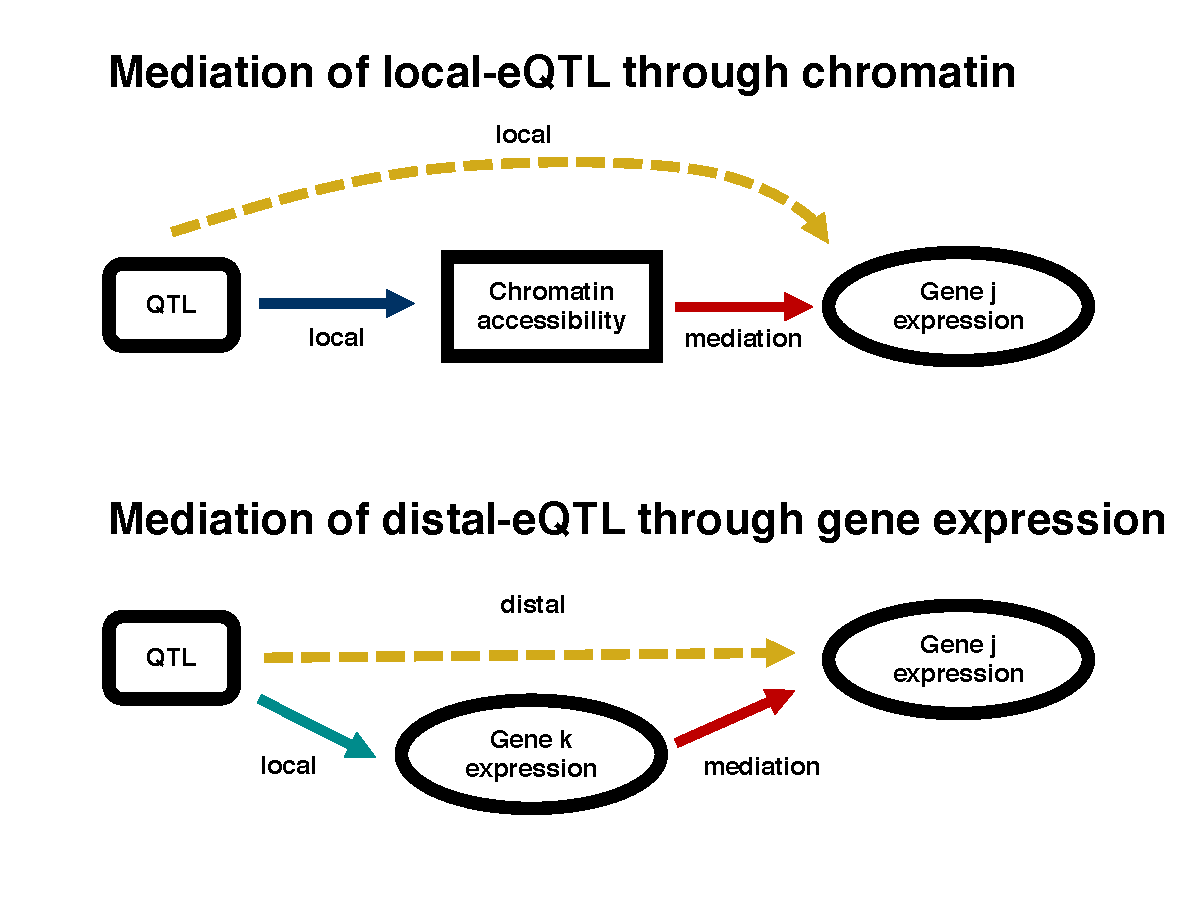
\includegraphics[width=\linewidth, page=1, clip, trim={0in 0.5in 0in 0in}]{figs/mediation_graph.pdf}
\caption{\textbf{Mediation models.} Simple mediation models for the genetic regulation of gene expression, in which local-eQTL are mediated through chromatin accessibility in the region of the gene,  and  distal-eQTL are mediated through the transcription of a proximal gene. Chromatin mediation is consistent with genetic variation influencing the accessibility of gene j to the transcriptional machinery. Mediation through proximal gene expression is consistent with distal-eQTL that result when the expression of gene j is dependent on a downstream interaction with gene k, such as transcription factors. \label{fig:graph}}
\end{figure}

\subsubsection{Genome-wide mediation.}

Mediation analysis have recently been used with genomic data, including in humans (\eg \citealt{Battle2014}). We use a similar approach to \cite{Chick2016} and \cite{Keller2018} to assess statistically significant mediation of eQTL effects on gene expression.

The mediation relationships are evaluated in a genome-wide  scan, allowing for the detection of FWER-corrected significant mediators that satisfy relationships \ref{rel:eQTL}, \ref{rel:cQTL}, and \ref{rel:full_mediator}. Similar to the QTL mapping genome scan described in Eq \ref{eq:alternative_model} and Eq \ref{eq:conditional_model}, the mediation scan involves a comparison of an alternative and a null model at loci across the genome. The alternative model is
\begin{equation}
y^{\text{G}_{j}}_{i} = \mu + \text{eQTL}_{i}^{\text{G}_{j}} + m_{ik} + \text{batch}_{i} + \varepsilon_{i},
\label{eq:mediation_alt}
\end{equation}
which is compared to the null model:
\begin{equation}
y^{\text{G}_{j}}_{i} = \mu + m_{ik} \nonumber + \text{batch}_{i} + \varepsilon_{i}
\label{eq:mediation_null}
\end{equation}
where $y^{\text{G}_{j}}_{i}$ is the expression levels for individual $i$ of gene $j$ with an eQTL, $\mu$ is the intercept term, $\text{eQTL}_{i}^{\text{G}_{j}}$ is the eQTL effect on gene $j$, $m_{ik}$ is the effect of the $k$\textsuperscript{th} mediator, either chromatin accessibility or gene expression depending on the mediation model being evaluated, $\text{batch}_{i}$ is the effect of the sequencing center, and $\varepsilon_{i}$ is random noise. Conditioned loci can be included for certain eQTL, as in Eq \ref{eq:conditional_model}, but not included here for clarity. Whereas with the QTL genome scan, the locus effect was changed at each position, for the mediation scan, it is fixed at the eQTL locus, and the mediator is changed.

Because the eQTL is always included in the alternative model but not the null model, the logP of the mediation scan should fluctuate around the observed eQTL logP. At mediators that possess some or all of the information present in the eQTL, the logP will drop. Significant logP drops represent candidate mediators. Significance thresholds to control FWER were determined by performing mediation scans on 1,000 permutations of the mediator variable. See \textbf{Appendix C} for greater detail on the mediation analysis, including permutation approach to significance thresholds and the formal criterion for mediation detection.

